%-------------------------------------------------------
% Introduction.tex
%
% This document contains the introduction of the paper
%-------------------------------------------------------
\section*{\small \textsc{I. introduction}}
The need for a new way for network management derives from several factors. The first is a change in traffic models. Actually, today's applications access different databases and servers before returning data to the end user device. This is in contrast to client-server applications, where the bulk of the communication occurs between one client and one server \cite{onf:sdn-description:traffic-models}. A second factor is the ``Consumerization of \ac{IT}''. Users are increasingly employing mobile personal devices such as smart phones, tablets and notebooks to access the corporate network. \ac{IT} is under pressure to accommodate these personal devices in a fine grained manner while protecting corporate/intellectual property and meeting compliance mandates \cite{onf:sdn-description:consumerization-IT}. Another aspect is the rise of cloud services. Enterprises have enthusiastically embraced cloud services resulting in unprecedented growth of these services. Enterprise business units now want the agility to access applications, infrastructures, and other \ac{IT} resources on demand \cite{onf:sdn-description:cloud}. Finally ``Big data'' means more bandwidth. Handling today's ``big data'' or mega datasets require massive parallel processing on thousands of servers, all of which need direct connections to each other \cite{onf:sdn-description:big-data}.

In addition, today's networks infrastructure presents some limitations. First, a complexity that leads to stasis. Actually, network technologies, nowadays, have always focused on designing protocols for connecting host reliably, with speed and with different network topologies on large distances. To meet business and technical needs, over the last few decades, the industry has evolved networking protocols to achieve higher performance, reliability, broader connectivity and stronger security. Protocols tend to be defined in isolation. Each solves a specific problem, without the benefit of any fundamental abstractions and this lead to stasis. This has also resulted in one of the primary limitations of today's networks: complexity \cite{onf:sdn-description:stasis}.

Second the need to change routers/switch configurations due to the use of virtualization \cite{ieee:sdn-and-virtualization} in cloud environment. Cloud is a dynamic environment where virtualization has become crucial. Actually, it has greatly increased the number of hosts requiring network connectivity and fundamentally altered assumptions about the physical location of hosts. Prior to virtualization, applications resided on a single server and primarily exchanged traffic with selected clients. Today instead, applications are distributed across multiple \ac{VM}, which exchange data flows with each other. \ac{VM} migrate to optimize and rebalance server workloads, causing the physical end points of existing flows to change (sometimes rapidly) over time. \ac{VM} migration challenges many aspects of traditional networking, from addressing schemes and name spaces to the basic notion of a segmented, routing-based design. These challenges make harder managing network configurations in real time.

Third, policy sometimes are inconsistent. To implement a network wide policy, \ac{IT} may have to configure thousands of devices and mechanisms. The complexity of today's network make it very difficult for \ac{IT} to apply consistent set of access, security, \ac{QoS} and other policies to increasingly mobile users, which leaves the enterprise vulnerable to security branches \cite{onf:sdn-description:policies}.

Another aspect is the slowness to scale. As demands on the data center rapidly grows, so too much the network grows. However, the network becomes vastly more complex with the addiction of hundreds or thousands of network devices that must be configured and managed \cite{onf:sdn-description:scale}.

Finally the last limitation is the dependency by single vendor. Carriers and enterprises seek to deploy new capabilities and services in rapid response to changing business needs or user demands. However, their ability to respond is hindered by vendor's equipment product cycles, which can range to three years or more. Lack of standard, open interfaces limits the ability of network operators to tailor the network to their individual environments \cite{onf:sdn-description:vendor-dependency}.

With the aim to overcome the above issues, industry and academic started to work on possible solutions. \acf{SDN} is one of such solutions. \ac{SDN} allows the construction of highly flexible and scalable networks that fit easily with the new business requirements.

\subsection*{\raggedright\small \textit{A. Outline}}
The paper is structured as: The following section introduces what is \ac{SDN} and the OpenFlow communication protocol. In section III we introduces network weakness using \ac{SDN} with the OpenFlow communication protocol and relative improvements. Finally we do our conclusion.
\section*{\small \textsc{II. \ac{SDN} and OpenFlow overview}}
\ac{SDN} is a new system architecture, that provides the ability to easily organize and management the network. The main goal is to separate the logic level where decisions are taken from the data that flows in the network. Actually the decision are taken in the control layer (also called \acf{CP}). While the data flow through the infrastructured layer (also called \acf{DP}) This high level vision, shown in Figure \ref{fig:sdn-and-openflow-overview:sdn-structure}, simplifies the network design and management.

\begin{figure}
\centering
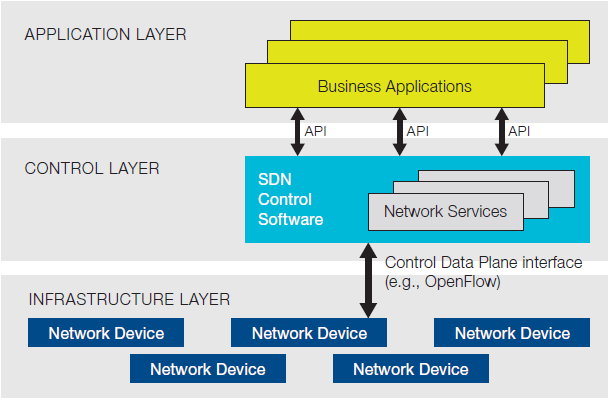
\includegraphics[scale=0.45]{Introduction/Image/SDNStructure.png}
\caption{\ac{SDN} structure}
\label{fig:sdn-and-openflow-overview:sdn-structure}
\end{figure}

The \ac{CP} is programmable with a higher level of abstraction and, as result, the network appears, to business applications, as a single point of exchange.
\ac{SDN} provides \acs{API} that allow the implementation of network services like routing, multicast, security, access control, bandwidth management, traffic engineering, \ac{QoS} and energy management.

The communication between the \ac{CP} and the \ac{DP} occurs through a communication protocol, the most famous one is the OpenFlow communication protocol \cite{onf:sdn-description:openflow}. With this protocol the \ac{CP} can exchange informations with the network devices in real-time.

There are several benefits from the use of \ac{SDN} architecture based on OpenFlow. First of all a centralized control of routers/switches multi vendor. Each vendor can implement the algorithm with its own logic but, in respect with the OpenFlow standard interface, multi vendor devices can receive the same directive. Second, a reduction of complexity through automation that derive from the previous point. This is possible because when an user program the control layer, automatically the rules are applied on each device. Third, an high rate of innovation. Finally, \ac{SDN} provides an higher level of reliability and security and a more granular level of control of entire network architecture.

The OpenFlow switch \cite{onf:openflow-specifications:switch-component} maintains by one or more \component{flow tables}, a \component{group table} and a \component{channel} for the external controller. OpenFlow compliant switches come in two types: \component{OpenFlow Only} and \component{OpenFlow Hybrid}. The first type supports only OpenFlow processing, all packets are processed by the OpenFlow pipeline. While the second supports also normal Ethernet switching operation like traditional L2 Ethernet switching, \acs{VLAN} isolation, L3 routing, \acs{ACL} and \ac{QoS} processing.

An OpenFlow switch contains a set of \component{flow tables} for pipeline processing, sequentially numbered starting at 0. Each table contains a set of flow rules. Each flow table entry specifies a set of operations that are applied, by the switch, in case of a match of an incoming packet.

Upon receiving a packet, a switch tries to match the packets against the flow rules present in the first \component{flow table} and this control can be positive or negative. In case of positive match the instruction set are applied to the packet, otherwise the switch applies the default actions (that are set when the device is first initialized).

The instruction set can include the following operations: forward a packet, update a field in the packet, group table processing (used for complex operation like multicast) and match the packet against the next flow table in the pipeline (for simplicity pipeline processing). Otherwise, default operations include: contact the controller asking for a role for the newly received flow, drop the packet or pipeline processing.